%==============================================================================
% Capítulo 5: Arquitectura del Sistema
%==============================================================================
\section{Arquitectura del sistema}\label{sec:arquitectura}

\subsection{Visión general}\label{subsec:vision-general}

El sistema propuesto se estructura como una arquitectura distribuida y modular compuesta por cinco capas claramente diferenciadas, siguiendo los principios de cohesión alta y acoplamiento bajo descritos por \textcite{Pressman2020_software_engineering}. En el diseño se previó proteger la comunicación con el exterior mediante TLS~1.2/1.3 a nivel de un proxy inverso (Nginx); la terminación TLS 1.2/1.3 se verifica de forma automatizada sobre el despliegue de referencia de la release v1.2.2 (prueba de humo de la \autoref{subsec:pruebas-automatizadas}, cuyo runbook se cita en el Anexo~\ref{sec:anexo-documentacion-operativa}; despliegue de referencia en el Anexo~\ref{sec:anexo-diagrama-arquitectura}), con certificado autofirmado de referencia; la campaña experimental usó dos despliegues, y la distinción es relevante: la medición telefónica del 5 y 6 de octubre de 2026 corrió sobre el perfil Compose aislado \texttt{corpus}, que no incluye el proxy inverso, mientras que la ingesta del brazo automático del 2 de octubre lo hizo sobre el stack base, que sí incluye Nginx con el certificado autofirmado de referencia; en ningún caso las mediciones de la \autoref{sec:resultados} dependen de TLS. En producción, el adoptante debe proveer un certificado emitido por una CA. La comunicación interna entre los servicios del sistema (N8N, backend, PostgreSQL) se realiza sobre la red aislada de Docker, que constituye el perímetro de confianza. Todas las interfaces entre capas utilizan el estilo arquitectónico REST con cuerpos JSON para el intercambio estructurado de datos \parencite{Fielding2002_rest}. Esta separación de responsabilidades facilita el reemplazo independiente de cualquier componente sin afectar a los demás.

La Tabla~\ref{tab:capas} sintetiza las cinco capas y sus responsabilidades específicas, y la Figura~\ref{fig:componentes} detalla la organización en capas del módulo de procesamiento.

\begin{table}[htbp]
\centering
\caption{Capas funcionales de la arquitectura del sistema}
\label{tab:capas}
\small
\begin{tabular}{@{}>{\raggedright\arraybackslash}p{3.0cm} >{\raggedright\arraybackslash}p{10.5cm}@{}}
\toprule
\textbf{Capa} & \textbf{Componentes y responsabilidades} \\
\midrule
1. Canales de entrada & Casilla de correo electrónico monitoreada mediante IMAP/SMTP, formulario web implementado como SPA React y número virtual de Twilio con transcripción automática del habla. \\
2. Orquestación & Motor N8N~2.11.2 desplegado en contenedor Docker autoalojado. Normaliza la entrada y coordina la invocación a las capas inferiores. \\
3. Procesamiento & Servicio Python sobre FastAPI~0.115 (configuración evaluada; Tabla~\ref{tab:configuracion-evaluada-entregada}) ejecutado bajo Uvicorn. Aplica clasificador híbrido en dos etapas (reglas + LLM) y expone una API REST documentada con OpenAPI~3.1. \\
4. Inferencia & Modelo Gemini~3.6 Flash de Google, invocado únicamente cuando el filtro determinístico previo no resuelve el caso (\autoref{subsec:subsistema-clasificacion}). \\
5. Persistencia & PostgreSQL~15.5 desplegado en contenedor con volumen persistente y respaldos diarios. Almacena los incidentes y la trazabilidad de cada decisión del clasificador. \\
\bottomrule
\end{tabular}
\par\smallskip
{\footnotesize\textit{Fuente:} elaboración propia.\par}
\end{table}

\begin{figure}[htbp]
\centering
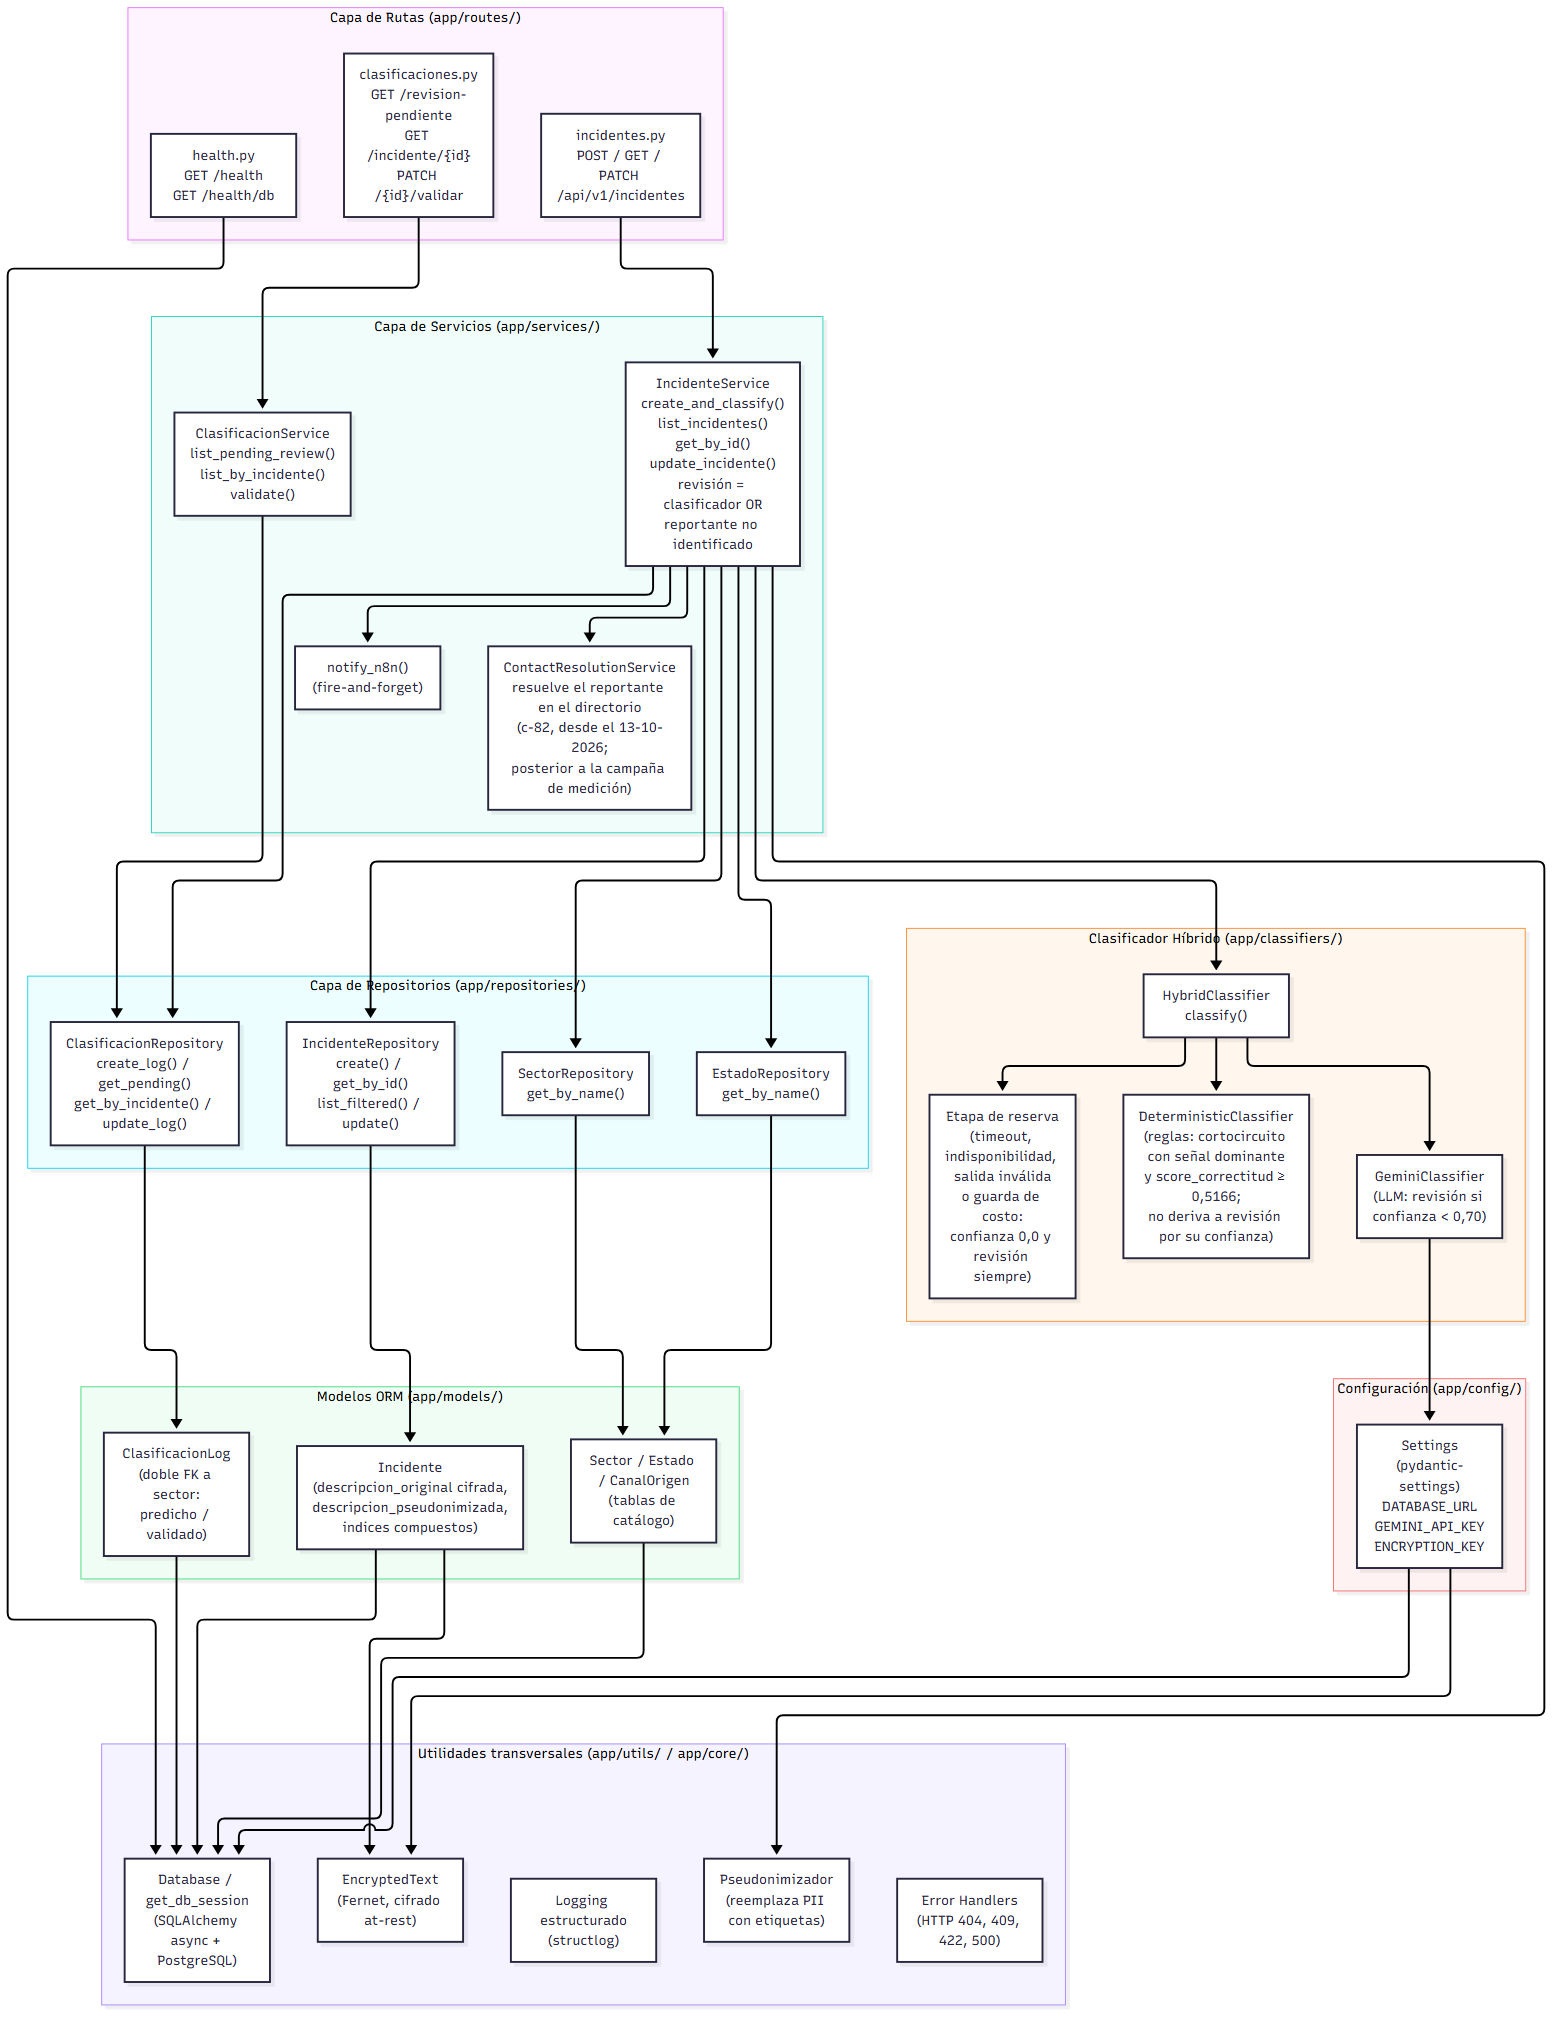
\includegraphics[width=0.80\textwidth,height=0.9\textheight,keepaspectratio]{componentes}
\caption[Diagrama de componentes del módulo Python organizado en capas]{Diagrama de componentes del módulo Python organizado en capas (routes, services, repositories, classifiers). Describe la configuración entregada (release \texttt{v1.2.5}): el filtro determinístico cortocircuita con señal dominante y puntaje de correctitud \(\geq 0{,}5166\) sin derivar por su confianza, la revisión por confianza menor que 0,70 rige solo sobre Gemini, la etapa de reserva deriva siempre, y el disparador por reportante no identificado en el directorio es posterior a la campaña (c-82, 13-10-2026; \autoref{tab:configuracion-evaluada-entregada}). Fuente: \texttt{docs/diagrams/componentes.md}.}
\label{fig:componentes}
\end{figure}

La trazabilidad operativa se garantiza mediante registros estructurados en cada capa, accesibles desde la capa de orquestación. La Figura~\ref{fig:arquitectura} representa esquemáticamente el flujo de información entre capas.

\begin{figure}[htbp]
\centering
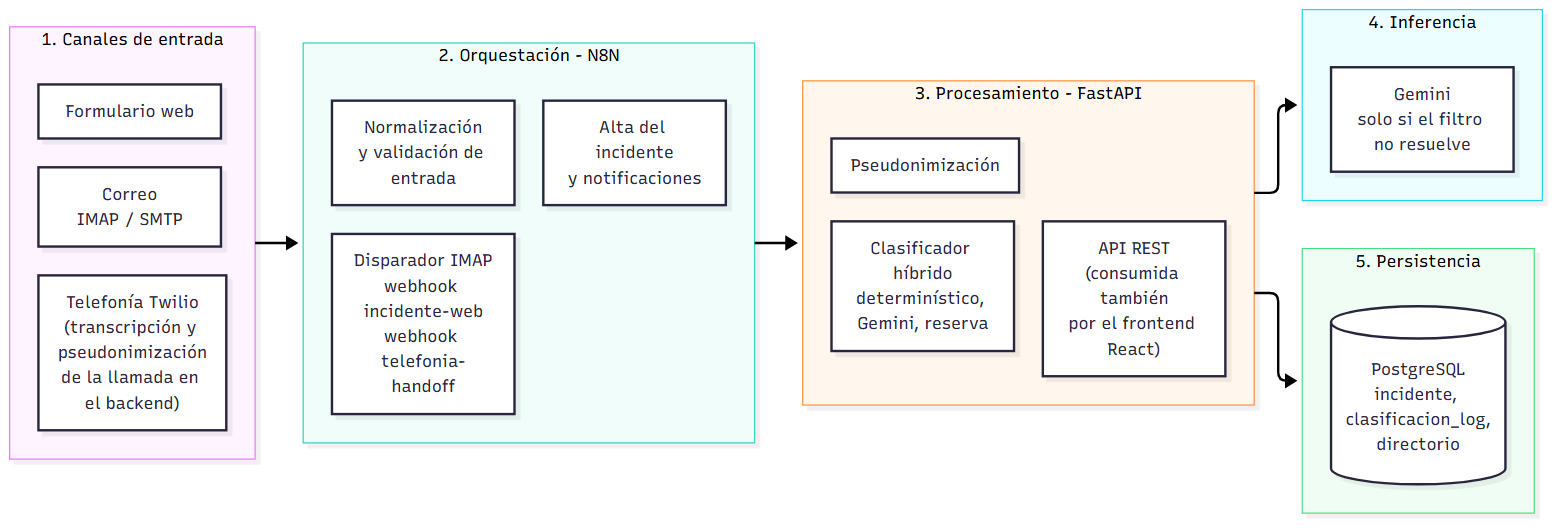
\includegraphics[width=\textwidth]{arquitectura_sistema}
\caption[Diagrama de arquitectura del sistema]{Diagrama de arquitectura del sistema: cinco capas y tres canales de entrada (correo, formulario web y telefonía), en la configuración entregada (release \texttt{v1.2.5}). Fuente versionada: \texttt{docs/diagrams/arquitectura\_sistema.md} (Anexo~\ref{sec:anexo-diagrama-arquitectura}).}
\label{fig:arquitectura}
\end{figure}

\begin{figure}[htbp]
\centering
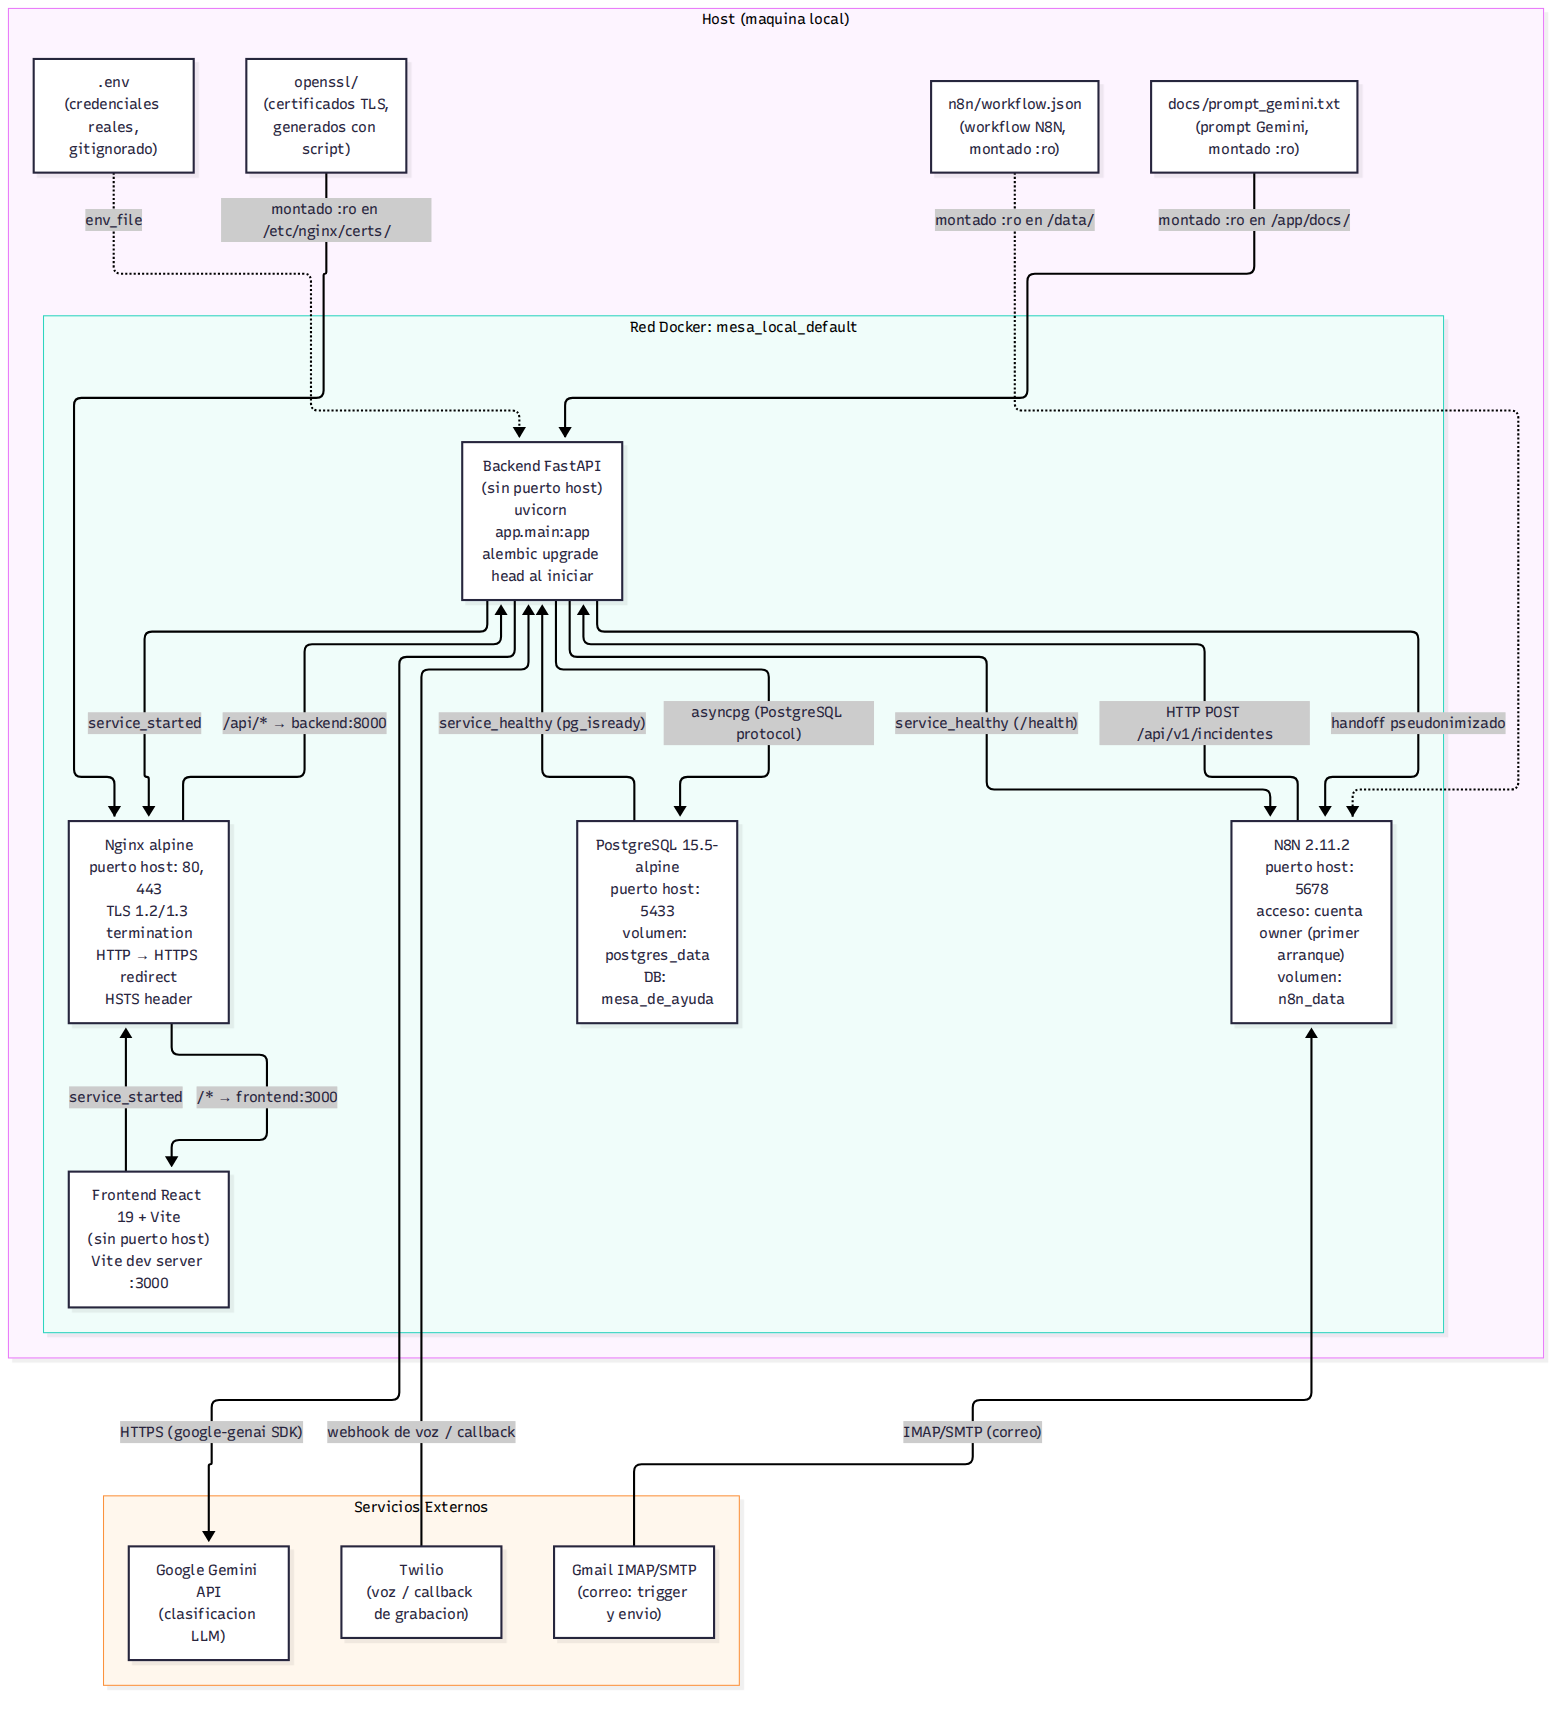
\includegraphics[width=0.92\textwidth]{despliegue}
\caption{Diagrama de despliegue del entorno local. Servicios, red Docker, volúmenes y servicios externos.}
\label{fig:despliegue}
\end{figure}

\begin{figure}[htbp]
\centering
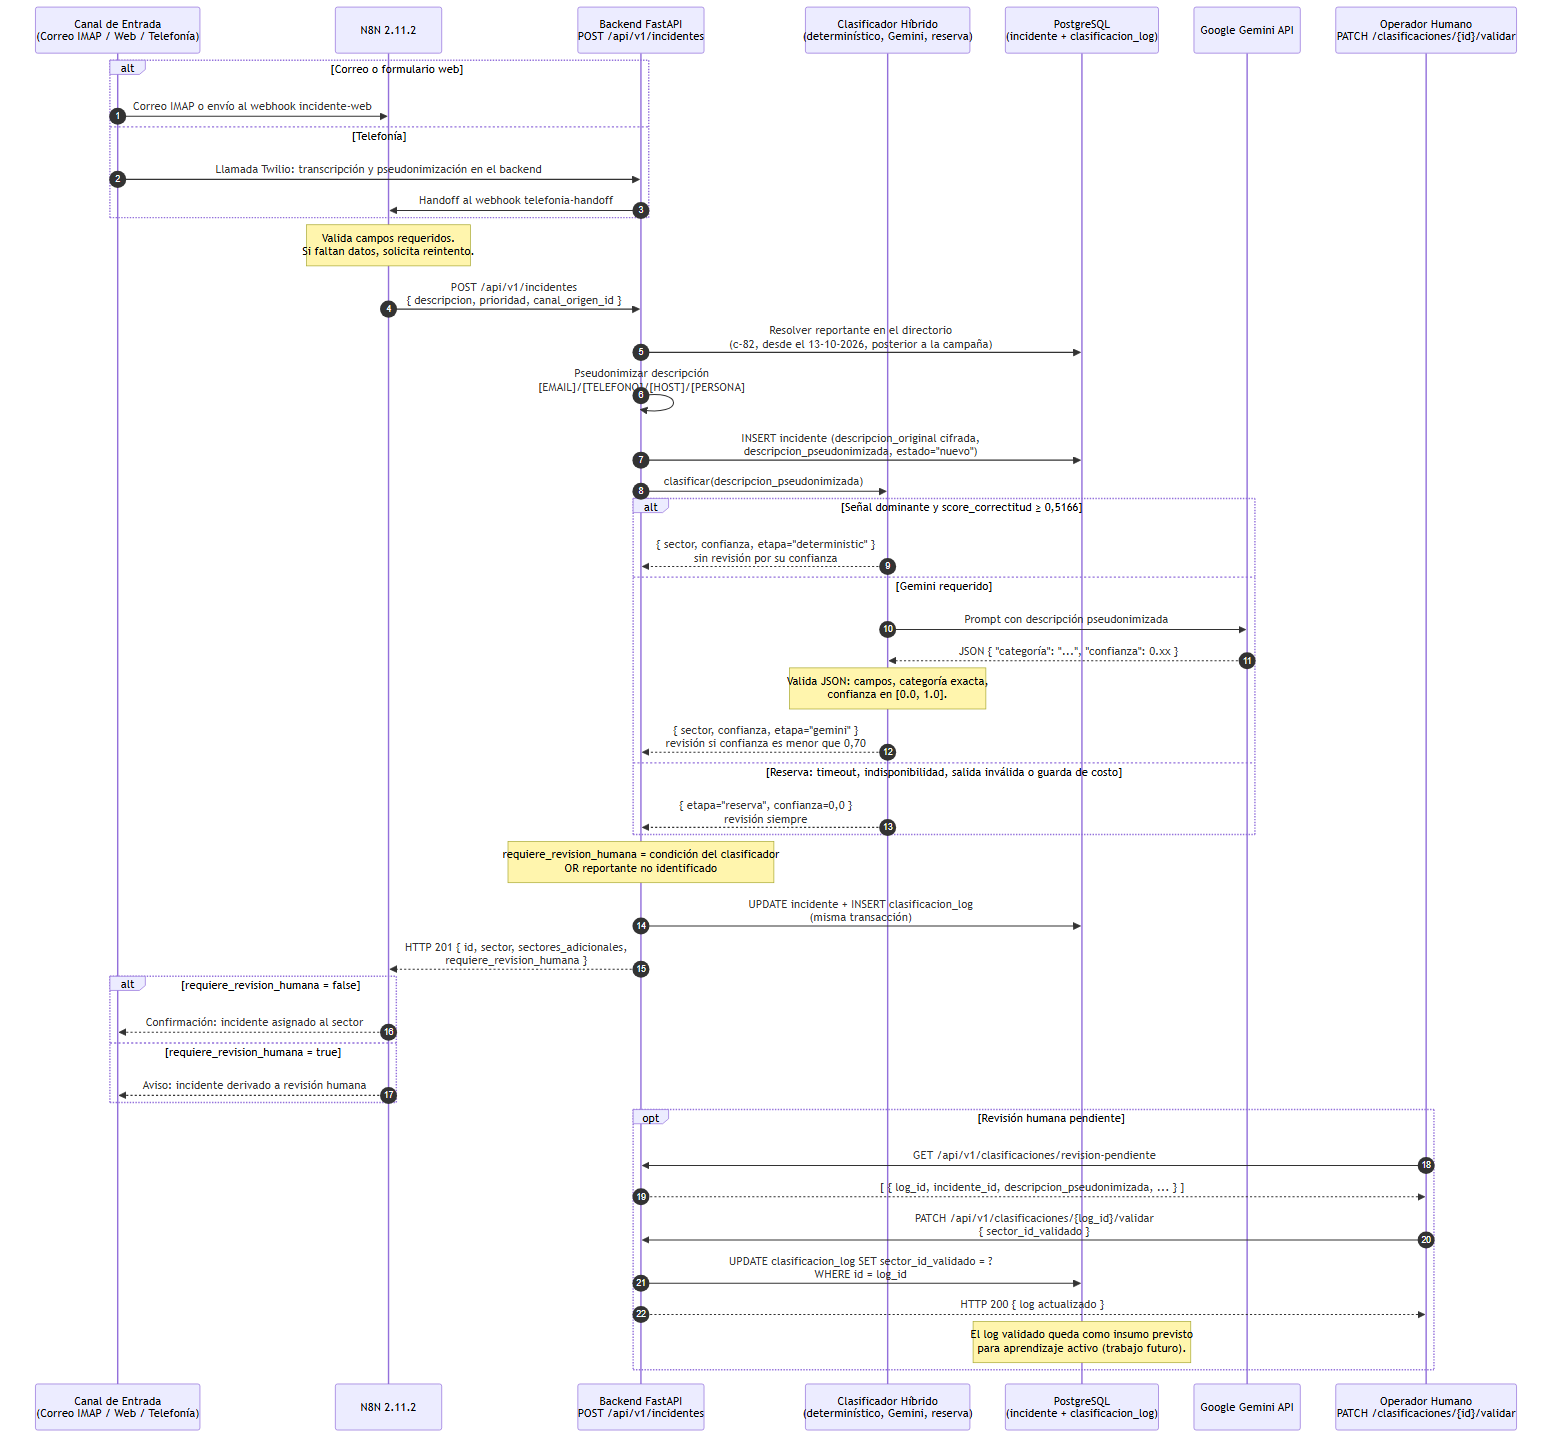
\includegraphics[width=\textwidth]{secuencia}
\caption[Diagrama de secuencia del flujo extremo a extremo de un incidente]{Diagrama de secuencia del flujo extremo a extremo de un incidente, desde el canal de entrada hasta la confirmación o la derivación a revisión humana, en la configuración entregada (release \texttt{v1.2.5}). El disparador por reportante no identificado en el directorio es posterior a la campaña (c-82, 13-10-2026): véase la \autoref{tab:configuracion-evaluada-entregada}.}
\label{fig:secuencia}
\end{figure}

\subsection{Capa de canales de entrada}\label{subsec:capa-canales}

La capa de canales de entrada habilita tres vías paralelas a través de las cuales un usuario puede reportar un incidente. La primera es el correo electrónico, monitoreado mediante IMAP/SMTP que detecta nuevos mensajes en una casilla institucional dedicada. La segunda vía es un formulario web implementado como aplicación React de página única (SPA) que se comunica directamente con la API REST del módulo de procesamiento. La autenticación se realiza mediante tokens JWT (JSON Web Tokens) con usuario y contraseña; la autenticación única corporativa (SSO) se prevé como evolución para entornos productivos (\autoref{sec:recomendaciones}). La tercera vía es la llamada telefónica, en la cual el usuario marca un número virtual provisto por Twilio, recibe instrucciones por voz pregrabadas y deja su solicitud; la grabación es transcrita automáticamente por el servicio de reconocimiento del habla del proveedor y enviada al flujo N8N mediante webhook posterior al cuelgue. El script TwiML que define el flujo de la llamada —incluyendo el mensaje de bienvenida en español rioplatense y la configuración de grabación— se implementa en el módulo de backend del proyecto (\texttt{app/cost\_guard/twiml.py}), versionado en el repositorio. Esta diversidad de canales amplía la accesibilidad del sistema y reduce las barreras al reporte oportuno.

\subsection{Capa de orquestación}\label{subsec:capa-orquestacion}

N8N actúa como orquestador principal del flujo de trabajo: recibe la entrada de cada canal, la normaliza en una estructura unificada y coordina la clasificación y la persistencia del incidente. La descripción operativa detallada del flujo ---los disparadores por canal, la estructura normalizada con identificador único (UUID v4), la invocación al módulo Python y la persistencia del ticket--- se desarrolla en la \autoref{subsec:construccion-flujo-n8n}. Los registros de cada ejecución se conservan durante 30 días para fines de auditoría y diagnóstico operativo; constituyen un conjunto de datos distinto de los incidentes, cuya retención se rige por la política declarada en la \autoref{subsec:principios-datos}.

\subsection{Capa de procesamiento}\label{subsec:capa-procesamiento}

El módulo de procesamiento se implementó como un servicio web ligero utilizando el marco FastAPI~0.115, expuesto sobre un servidor ASGI Uvicorn 0.30.6 (versiones de la configuración evaluada; Anexo~B, Tabla~\ref{tab:configuracion-evaluada-entregada}) \parencite{Tiangolo2024_fastapi}. La elección de FastAPI obedece a su soporte nativo de validación de esquemas mediante Pydantic, su rendimiento competitivo y su documentación automática conforme a la especificación OpenAPI~3.1.

Las dependencias del módulo se organizan por capas funcionales claramente delimitadas. La capa de acceso a datos utiliza SQLAlchemy~2.0 como mapeador objeto-relacional (ORM) y asyncpg como driver asincrónico para PostgreSQL, en coherencia con la operación no bloqueante de FastAPI. La capa de procesamiento textual emplea las bibliotecas regex y unicodedata de la biblioteca estándar de Python para normalización ortográfica y eliminación de signos diacríticos. La capa de inferencia se comunica con la interfaz oficial del modelo \texttt{gemini-3.6-flash} mediante el cliente google-genai >=2.20.0 de la configuración evaluada (SDK unificado de Google Generative AI), con los siguientes parámetros de configuración: temperatura \(= 0{,}3\), top\_p \(= 0{,}9\), max\_tokens \(= 100\) y timeout \(= 30\)~s por intento del backend al modelo, con un presupuesto total de \(60\)~s por clasificación. Estos valores corresponden a la configuración adoptada para el despliegue y no a un procedimiento de optimización documentado; su calibración sistemática frente a valores alternativos se plantea como trabajo futuro (\autoref{sec:recomendaciones}). Las bibliotecas NumPy~2.1 y Pandas~2.2 se utilizan exclusivamente para la generación de reportes agregados de desempeño y no participan del flujo de procesamiento individual de incidentes.

\subsection{Subsistema de clasificación híbrido}\label{subsec:subsistema-clasificacion}

El subsistema de clasificación adopta un enfoque híbrido en dos etapas, característica que lo diferencia de aproximaciones puramente basadas en modelo externo. La primera etapa aplica un filtro determinístico basado en expresiones regulares y diccionarios de términos del dominio. La procedencia de los datos empleados para construir el filtro determinístico, redactar las reglas de frontera del prompt y fijar el punto de operación se declara en la \autoref{subsec:interpretacion-resultados}. La especificación detallada del prompt y de los parámetros de configuración del modelo se documenta en el Anexo~H.

Este filtro resuelve de inmediato los incidentes con marcadores léxicos inequívocos y emite dos magnitudes en \([0;1]\) que no son probabilidades de acierto: la \emph{confianza}, índice de fuerza de señal ---margen del sector ganador sobre el segundo, ponderado por la cantidad de patrones coincidentes--- que vale 0 con menos de dos patrones, y el \emph{puntaje de correctitud} (\texttt{score\_correctitud}), que ordena la correctitud esperada. El filtro decide sin consultar al modelo (cortocircuito) cuando la señal es dominante ---sin empate ni ausencia de coincidencias--- y el puntaje alcanza el punto de operación 0,5166; la confianza no interviene y esos casos no se derivan a revisión por su confianza. El punto se derivó por validación cruzada de cinco pliegues sobre el corpus, maximizando la cobertura sin que la precisión del filtro fuera inferior a la del modelo sobre el conjunto que resuelve (0,7385 frente a 0,6769 sobre los 130 casos con predicción de ambas etapas, ambas estimadas dentro de la muestra; \autoref{subsec:sensibilidad-ajustes}), y equivale a resolver los 131 casos con señal dominante.

La segunda etapa, activada únicamente cuando el filtro determinístico no resuelve el caso, consulta al modelo Gemini~3.6 Flash mediante un prompt estructurado en español que incluye una breve descripción de cada categoría, ejemplos representativos balanceados y la solicitud explícita de devolver la categoría asignada y un valor numérico de confianza entre 0 y 1 en formato JSON estricto. El diseño compositivo reserva la capacidad semántica del modelo para los casos que el filtro no resuelve, lo que reduce la latencia y el costo de inferencia. El pipeline completo comprende tres etapas, aplicadas en orden: (1)~el filtro determinístico, (2)~el modelo Gemini y (3)~una etapa de reserva (\emph{fallback}) que, cuando el modelo no responde o no produce una salida válida, fija la confianza en 0,0 y marca siempre el caso para revisión humana. La regla \texttt{requiere\_revision\_humana = (confianza < 0{,}70)} se evalúa solo sobre la salida de la etapa Gemini; la etapa de reserva deriva siempre a revisión, con confianza 0,0, y la etapa determinística no deriva por su confianza. Desde el 13 de octubre de 2026, posterior a las corridas de la campaña, el backend deriva además a revisión el incidente cuyo reportante no se identifica en el directorio de empleados, condición independiente de la clasificación. El desglose de casos resueltos por cada etapa del pipeline sobre el corpus de validación se reporta en la \autoref{sec:resultados}.

El camino de clasificación es único para los tres canales de entrada. Tanto el correo electrónico y el formulario web como la llamada telefónica resuelven su sector mediante esta misma cascada híbrida, aplicada sobre la descripción pseudonimizada del incidente: ningún canal aporta una clasificación precalculada que omita la cascada, de modo que las reglas determinísticas, el prompt y las reglas de frontera se ajustan una sola vez para todo el sistema. El prompt único incorpora reglas de desambiguación de frontera entre sectores adyacentes (acceder o iniciar sesión en una aplicación se orienta a Soporte Tecnico Software; la digitalización, el escáner o la impresora se orientan a Soporte Tecnico Hardware; el servidor, la red, SMTP o una VM se orientan a Sistemas). Desde el punto de vista del costo, la clasificación telefónica dejó de computarse sobre una invocación incondicional al modelo externo: el canal atraviesa el filtro determinístico y solo escala al modelo semántico cuando la cascada lo requiere.

\subsection{Modelo de datos}\label{subsec:modelo-datos}

La persistencia se realiza sobre PostgreSQL~15.5, desplegado en contenedor Docker bajo configuración de respaldo diario y replicación física opcional para entornos productivos \parencite{PostgreSQL2024_docs}. El modelo de datos se organiza alrededor de siete entidades principales, descritas en la Tabla~\ref{tab:entidades}.

\begin{table}[htbp]
\centering
\caption[Entidades principales del modelo de datos]{Entidades principales del modelo de datos de la configuración entregada (release \texttt{v1.2.5}); el atributo \texttt{reportante\_empleado\_id}, el cuarto rol del directorio y el cifrado del contacto son posteriores a la campaña de medición (c-82, c-86 y c-153).}
\label{tab:entidades}
\footnotesize\singlespacing
\begin{tabular}{@{}>{\raggedright\arraybackslash}p{3.4cm} >{\raggedright\arraybackslash}p{5.3cm} >{\raggedright\arraybackslash}p{6.9cm}@{}}
\toprule
\textbf{Tabla} & \textbf{Atributos clave} & \textbf{Descripción} \\
\midrule
\texttt{incidente} & id (PK), descripcion\_original (cifrada), descripcion\_pseudonimizada, prioridad, sector\_id (FK), estado\_id (FK), canal\_origen\_id (FK), reportante\_empleado\_id (FK), requiere\_revision\_humana & Tabla central: descripción original cifrada en reposo y descripción pseudonimizada, prioridad, sector asignado, estado actual, canal de origen, reportante resuelto en el directorio e indicador de revisión humana. \\
\texttt{sector} & id (PK), nombre & Catálogo de los cinco sectores canónicos: Seguridad Informatica, Soporte Tecnico Hardware, Soporte Tecnico Software, Bases de Datos y Sistemas. \\
\texttt{estado} & id (PK), nombre, es\_terminal & Catálogo de estados: nuevo, en proceso, en espera, resuelto y cerrado. \\
\texttt{canal\_origen} & id (PK), nombre & Catálogo de canales: correo, formulario web y llamada telefónica. \\
\texttt{clasificacion\_log} & id (PK), incidente\_id (FK), sector\_id\_predicho (FK), sector\_id\_validado (FK), confianza, etapa, requiere\_revision\_humana & Registro de cada decisión del clasificador, con el sector predicho, la confianza asociada, la etapa que resolvió, el indicador de revisión y el sector validado por el sector responsable. \\
\texttt{users} & id (PK), username (UNIQUE), hashed\_password, is\_active & Almacena credenciales de operadores para autenticación JWT. \\
\texttt{directorio\_empleado} & id (PK), legajo (UNIQUE), nombre, email y telefono (cifrados), email\_bidx (UNIQUE), telefono\_bidx, sector\_id (FK), rol, activo, fecha\_baja, user\_id (FK) & Directorio institucional de empleados para resolución de contacto y notificación. El correo y el teléfono se cifran en reposo con Fernet y se buscan mediante un índice ciego (HMAC-SHA-256), según la decisión de c-153; el campo \texttt{rol} admite cuatro valores: usuario final, mesa de ayuda, administrador del directorio y gestión de incidentes. La columna \texttt{fecha\_baja} registra la desactivación y sostiene la retención (relación laboral activa más un año). \\
\bottomrule
\end{tabular}
\par\smallskip
{\footnotesize\textit{Fuente:} elaboración propia a partir de \texttt{App/Backend/app/models/}.\par}
\end{table}

El canal de origen constituye una entrada opcional del backend: el esquema de creación de incidentes acepta \texttt{canal\_origen\_id} como campo anulable, de modo que un incidente puede registrarse sin canal conocido. La entidad central \texttt{incidente} referencia mediante claves foráneas a los catálogos de sector, estado y canal de origen, y mantiene una relación uno a muchos con \texttt{clasificacion\_log} para preservar la trazabilidad histórica de las decisiones del clasificador. El número de incidente que se comunica al usuario corresponde al identificador único del registro, formateado para su legibilidad; la incorporación de un prefijo configurable se prevé como evolución futura (\autoref{sec:recomendaciones}). El esquema completo, incluyendo restricciones de integridad referencial e índices secundarios, se documenta en el Anexo~C. El directorio de empleados (\texttt{directorio\_empleado}) se vincula opcionalmente con la tabla de autenticación mediante \texttt{user\_id} y referencia el catálogo de sectores mediante \texttt{sector\_id}; su campo \texttt{rol} distingue al usuario final, a la mesa de ayuda, al administrador del directorio y a la gestión de incidentes (cuatro valores; \autoref{tab:entidades}).

\begin{figure}[htbp]
\centering
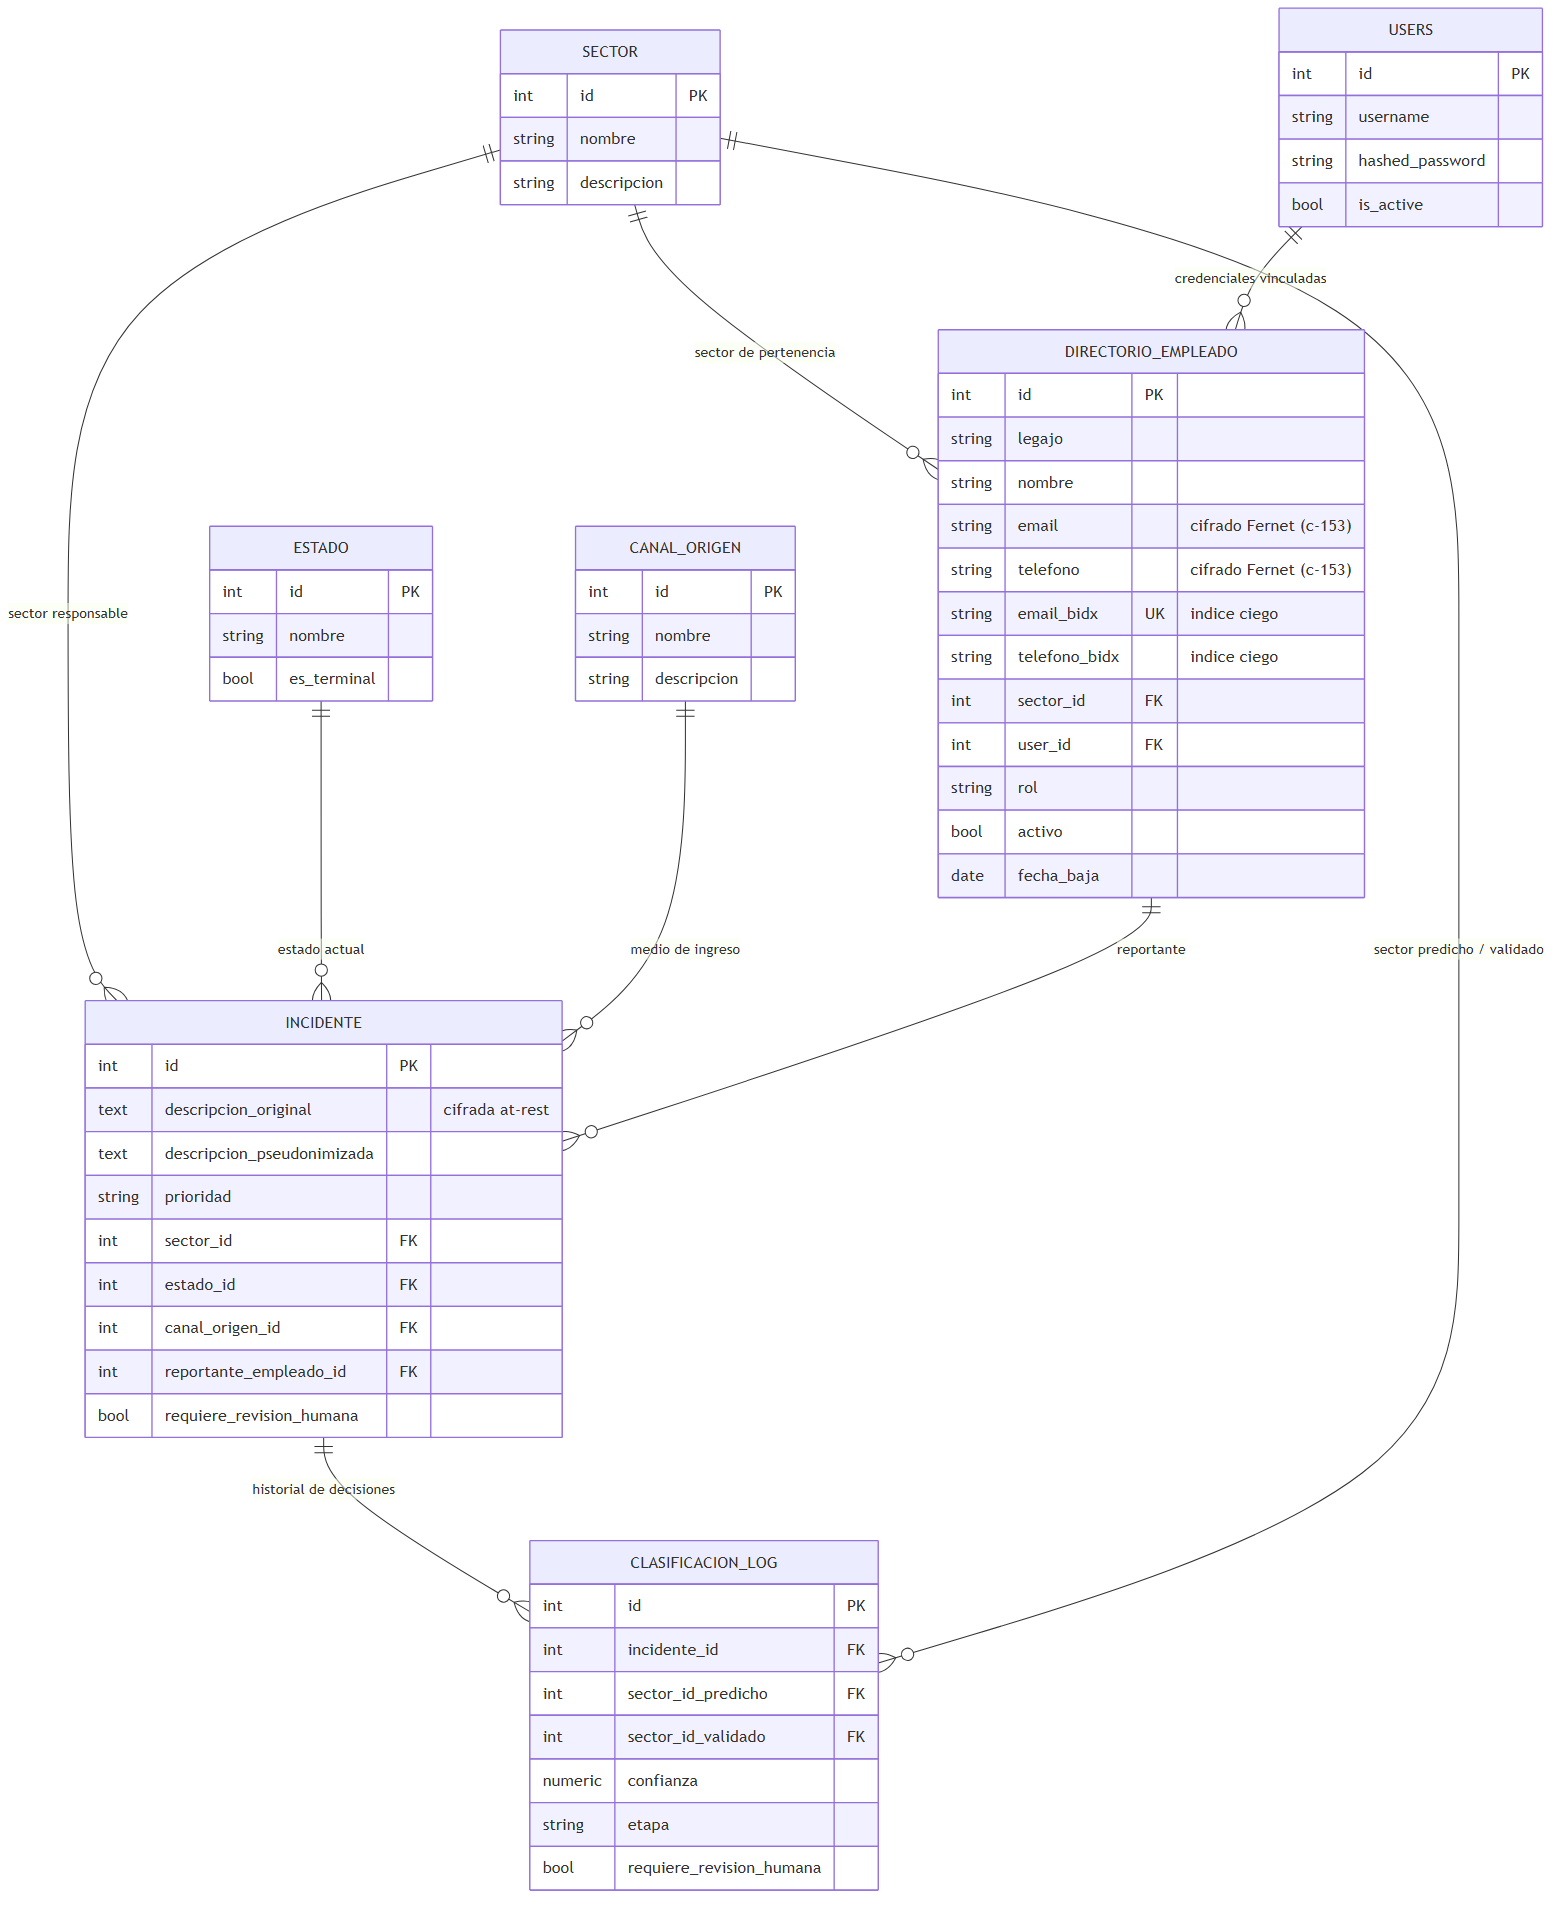
\includegraphics[width=0.85\textwidth]{er_modelo_datos}
\caption[Diagrama entidad-relación de las siete entidades principales]{Diagrama entidad-relación de las siete entidades principales del modelo de datos de la configuración entregada (release \texttt{v1.2.5}; esquema completo en el Anexo~C).}
\label{fig:er_modelo_datos}
\end{figure}

\subsection{Contrato de la interfaz REST}\label{subsec:contrato-rest}

La interfaz de programación de aplicaciones expuesta por el módulo Python sigue el estilo arquitectónico REST \parencite{Fielding2002_rest}, con representación de recursos mediante identificadores uniformes, uso semántico de los métodos HTTP estándar y comunicación sin estado del lado del servidor. La autenticación se realiza mediante tokens JWT (JSON Web Tokens) firmados con HS256, validados en cada solicitud mediante el esquema OAuth2PasswordBearer de FastAPI. La Tabla~\ref{tab:api} sintetiza los principales puntos de entrada.

\begin{table}[htbp]
\centering
\caption{Puntos de entrada principales de la interfaz REST}
\label{tab:api}
\small
\begin{tabular}{@{}p{1.8cm} >{\raggedright\arraybackslash}p{5.2cm} p{1.8cm} >{\raggedright\arraybackslash}p{4.8cm}@{}}
\toprule
\textbf{Método} & \textbf{Ruta} & \textbf{Código} & \textbf{Función} \\
\midrule
\multicolumn{4}{@{}l}{\textbf{Autenticación}} \\
POST & \texttt{/api/v1/auth/login}, \texttt{/refresh}, \texttt{/logout} & 200 OK & Inicio y renovación de sesión y cierre de sesión de operadores. \\
GET & \texttt{/api/v1/auth/me} & 200 OK & Recupera el perfil del operador autenticado. \\
\midrule
\multicolumn{4}{@{}l}{\textbf{Incidentes}} \\
POST & \texttt{/api/v1/incidentes} & 201 Created & Crea un nuevo ticket y devuelve el identificador generado. \\
GET & \texttt{/api/v1/incidentes/\{id\}} & 200 OK & Recupera la información de un ticket por su identificador. \\
PATCH & \texttt{/api/v1/incidentes/\{id\}} & 200 OK & Actualiza los campos editables de un ticket. \\
\midrule
\multicolumn{4}{@{}l}{\textbf{Clasificaciones}} \\
GET & \texttt{/api/v1/clasificaciones/incidente/\{id\}} & 200 OK & Recupera la trazabilidad de la clasificación de un incidente. \\
GET & \texttt{/api/v1/clasificaciones/revision-pendiente} & 200 OK & Lista los casos derivados a revisión humana. \\
PATCH & \texttt{/api/v1/clasificaciones/\{log\_id\}/validar} & 200 OK & Registra la categoría validada por el sector responsable. \\
\midrule
\multicolumn{4}{@{}l}{\textbf{Estadísticas}} \\
GET & \texttt{/api/v1/estadisticas/resumen}, \texttt{/tendencias} & 200 OK & Agregados y series temporales para el dashboard. \\
\midrule
\multicolumn{4}{@{}l}{\textbf{Salud}} \\
GET & \texttt{/health} y \texttt{/health/db} & 200 OK & Verificación de salud del servicio para monitoreo externo. \\
\bottomrule
\end{tabular}
\par\smallskip
{\footnotesize\textit{Fuente:} elaboración propia.\par}
\end{table}

Los códigos de estado HTTP se utilizan conforme a su semántica original: 201 cuando un recurso se crea exitosamente, 200 cuando una consulta se atiende con éxito, 400 cuando los datos de entrada no validan el esquema esperado, 401 cuando la autenticación falla, y 500 cuando ocurre un error interno no recuperable. La Tabla~\ref{tab:api} no es exhaustiva: reúne los grupos principales de puntos de entrada, mientras que el contrato completo de la interfaz ---que comprende la totalidad de las rutas expuestas--- se documenta en el Anexo~D y se versiona en \texttt{docs/openapi.json}; la especificación OpenAPI~3.1 la genera FastAPI automáticamente.

\newpage
